% science_template.tex
% See accompanying readme.txt for copyright statement, change log etc.

% Any modification of this template, including writing a paper using it,
% MUST rename the file i.e. use a different file name.

%%%%%%%%%%%%%%%% START OF PREAMBLE %%%%%%%%%%%%%%%

% Basic setup. Authors shouldn't need to adjust these commands.
% It's annoying, but please do NOT strip these into a separate file.
% They need to be included in this .tex for our production software to work.

% Use the basic LaTeX article class, 12pt text
\documentclass[12pt]{article}

% Science uses Times font. If you don't have this installed (most LaTeX installations will be
% fine) or prefer the old Computer Modern fonts, comment out the following line
\usepackage{newtxtext,newtxmath}
% Depending on your LaTeX fonts installation, you might get better results with one or both of these:
%\usepackage{mathptmx}
%\usepackage{txfonts}

% Allow external graphics files
\usepackage{graphicx}

% Use US letter sized paper with 1 inch margins
\usepackage[letterpaper,margin=1in]{geometry}

% Double line spacing, including in captions
\linespread{1.5} % For some reason double spacing is 1.5, not 2.0!

% One space after each sentence
\frenchspacing

% Abstract formatting and spacing - no heading
\renewenvironment{abstract}
	{\quotation}
	{\endquotation}

% No date in the title section
\date{}

% Reference section heading
\renewcommand\refname{References and Notes}

% Figure and Table labels in bold
\makeatletter
\renewcommand{\fnum@figure}{\textbf{Figure \thefigure}}
\renewcommand{\fnum@table}{\textbf{Table \thetable}}
\makeatother

% Call the accompanying scicite.sty package.
% This formats citation numbers in Science style.
\usepackage{scicite}

% Provides the \url command, and fixes a crash if URLs or DOIs contain underscores
\usepackage{url}

%%%%%%%%%%%% CUSTOM COMMANDS AND PACKAGES %%%%%%%%%%%%

% Authors can define simple custom commands e.g. as shortcuts to save on typing
% Use \newcommand (not \def) to avoid overwriting existing commands.
% Keep them as simple as possible and note the warning in the text below.
% Example:
\newcommand{\bb}[1]{\mathbf{#1}}
\newcommand{\B}[1]{\mathbb{#1}}
\graphicspath{{plots}}

% Please DO NOT import additional external packages or .sty files.
% Those are unlikely to work with our conversion software and will cause problems later.
% Don't add any more \usepackage{} commands.


%%%%%%%%%%%%%%%% TITLE AND AUTHORS %%%%%%%%%%%%%%%%

% Title of the paper.
% Keep it short and understandable by any reader of Science.
% Avoid acronyms or jargon. Use sentence case.
\def\scititle{%
  Can you ``buy'' an American presidential election?
}
% Store the title in a variable for reuse in the supplement (otherwise \maketitle deletes it)
\title{\bfseries \boldmath \scititle}

% Author and institution list.
% Institution numbers etc. should be hard-coded, do *not* use the \footnote command.
\author{
	% You can write out first names or use initials - either way is acceptable, but be consistent
  Johann D.~Gaebler$^{1,\ast}$,
  Andrew Gelman$^{2}$,
  Sharad Goel$^{3}$,
  Todd Rogers$^{3}$\and
	% Additional lines of authors should be inserted using the \and command (not \\)
	% Institution list, in a slightly smaller font
	\small$^{1}$Dept.\ of Statistics, Harvard University, Cambridge, MA 02138, USA.\and
	\small$^{2}$Depts. of Statistics and Political Science, Columbia University, New York, NY 10027, USA.\and
  \small$^{3}$Harvard Kennedy School, Harvard University, Cambridge, MA 02138, USA.\and
	% Identify at least one corresponding author, with contact email address
	\small$^\ast$Corresponding author. Email: jgaebler@fas.harvard.edu.
}

%%%%%%%%%%%%%%%%% END OF PREAMBLE %%%%%%%%%%%%%%%%


%%%%%%%%%%%%%%%% START OF MAIN TEXT %%%%%%%%%%%%%%%
\begin{document} 

% Insert the title and author list
\maketitle

\noindent
Different kinds of competition have historically limited the influence of money
in American politics. Competition among multitudes of ideologically motivated
small donors mitigate special interests’ abilities to transactionally ``invest''
in campaigns~\cite{ansolabehere2003why}. Interest groups also compete directly
with each other to control valuable government
resources~\cite{grossman1994protection, ferguson1995golden}, and parties compete
to raise funds~\cite{stromberg2008how}. As a result, it is difficult for one
party’s fundraising to dominate the other’s. Institutional and cultural factors
also limit the role of money in politics. Laws and norms against
\emph{quid pro quo} arrangements diminish how much donors can get in return for
transactional campaign contributions~\cite{buckley1976}. Disproportionate
campaign spending can also benefit the other party when it becomes an issue in
its own right, as in Wisconsin’s recent supreme court
election~\cite{epstein2025liberal}---the most expensive judicial race in U.S.
history.

But important changes in the structure of American politics threaten to disrupt
this equilibrium, heightening concerns that elections can be ``bought.'' The
Supreme Court’s 2010 ruling in \emph{Citizens United v. FEC} paved the way for
large donors to finance national campaigns~\cite{citizens2010}. The top 50
donors to 2024 U.S. federal elections collectively contributed over \$2 billion,
with the largest individual donor giving nearly \$300 million
\cite{opensecrets2024top}. At the same time, the number of potential
``megadonors'' has risen: only eight Americans could have individually funded
the \$1.2 billion cost of the 1984 federal election cycle~\cite{forbes1984,
alexander1988financing}, compared to more than 100 who could have covered the
\$16 billion spent in 2024~\cite{lafranco2025forbes, opensecrets2024total}.
Additionally, presidential elections have grown much closer in recent decades,
lowering the cost of swinging an election: Whereas three of the five elections
in the 1970s and 80s were decided by double-digit popular vote margins, six of
the last seven elections were won by less than five percentage
points~\cite{gelman2014twentieth}.

Here we investigate the risk of election ``buying.'' To do so, we first estimate
how much a candidate could improve their chances of winning by strategically
increasing their support by, for example, 500,000 votes across battleground
states. Then we estimate the cost of implementing such campaign strategies.
While reasoning about these strategies—which go beyond the scale of typical
efforts—is inherently uncertain, this exercise helps us understand the potential
risk of large donors to America’s democratic integrity.

\section*{Margins of victory are predictably small}

Consistent with many political observers’ expectations, the 2024 presidential
election was close, with a national vote margin of only 1.4 percentage points. A
swing of 230,000 votes won by Democrats in a handful of swing states would have
flipped the election outcome: 120,000 in Pennsylvania, 80,000 in Michigan, and
30,000 in Wisconsin. But it was less obvious ahead of time that it would be
close in this particular way. In November 2024, the Cook Political Report, a
widely-regarded election handicapping firm, listed seven states as potential
``tossups''~\cite{cpr2024electoral}. One might have needed additional votes in
all these battleground states, rather than simply the three that ended up being
pivotal, to have materially improved the campaigns’ chances of winning.

To account for this uncertainty, we start with the election forecasting model
from the \emph{Economist} magazine~\cite{gelman2024grappling} that used data
from national and state-level polls, prior elections, and economic fundamentals.
The model yields simulations representing the joint forecast of the vote margins
in the fifty states. Using these simulations, we then estimate how much each
party can increase its \emph{ex ante} chance of victory by, for example,
obtaining 500,000 additional supporters—assuming those additional votes are
strategically obtained in states to maximize a party’s probability of winning
under the model. Concretely, we frame the problem as a mixed-integer program,
which we numerically solve. We use the forecast from October 1, 2024, roughly a
month before the election, to ensure parties can enact the type of campaign
strategies this exercise produces. (See the SI for optimization and modeling
details.)

At the time of the forecast, Kamala Harris and Donald Trump were estimated to
have 55\% and 45\% chances of winning the electoral vote.
Fig.~\ref{fig:efficiency} plots how these probabilities increase for each
candidate under a roughly optimal vote-getting strategy. To ensure the
strategies are both simple and realistic, we require a candidate to receive at
least 10,000 additional voters in any state where the campaign deploys
resources, and we cap the maximum increase in votes at 5\% of a state’s actual
turnout in the 2024 election. We find that around 100,000 additional voters
would boost both campaigns’ win probabilities by slightly less than 10
percentage points. A 70\% chance of victory requires around 250,000 additional
voters for Democrats, or around 500,000 for Republicans; with 500,000 additional
votes, Democrats could raise their probability of winning to over 80\%. This
analysis assumes the \emph{net} votes (i.e., the \emph{difference} between the
numbers of votes candidates receive) would increase by the stated amount.
Accomplishing that result might require recruiting many more voters, as efforts
to obtain voters in one party would likely be matched in part by efforts to
obtain those in the other party—a point we return to below.

Our analysis indicates that most of the additional net votes—under these
optimized strategies—should come from a small number of swing states. For
example, assuming a party could optimally gain 500,000 net votes, Fig. 2
illustrates the optimal geographic allocation for Democrats and Republicans
conditional on the publicly-available forecast. For Democrats, the additional
votes would be concentrated in Pennsylvania ~190,000), Michigan~(140,000), and
Wisconsin~(110,000); for Republicans, in Michigan~(180,000) and
Pennsylvania~(150,000), along with smaller blocs in Nevada~(40,000), New
Hampshire~(40,000), Arizona~(30,000), and Wisconsin~(20,000). These differences
represent real changes in vote counts, but are within the range of election to
election fluctuations.

\section*{How much do additional net votes cost?}

We next gauge the cost of gaining several hundred thousand net votes spread
across a handful of states. Campaigns could employ a variety of methods for
increasing their vote margins, ranging from advertising, to registration drives,
to mobilization efforts that remind voters to cast a ballot or that may even
transport them to the polls~\cite{green2023get}. Recent elections have also seen
the development of unconventional and legally questionable tactics such as voter
roll purges, voter intimidation, and lotteries for registered
voters~\cite{schleifer2024musk}.

Parties can increase their margins by persuasion, mobilization of supporters,
and de-mobilization of supporters on the other side. The cost of voter
mobilization varies based on mode of contact (e.g., television ads, direct mail,
or canvassing), type of election (e.g., presidential, midterm, or mayoral), and
location. Though these studies have produced a wide range of estimates,
published numbers generally do not exceed \$1,000 per vote and are typically far
less. For instance, in a meta-analysis of almost 60 canvassing RCTs, Green \&
Gerber~\cite{green2023get} estimate an average cost per vote of around \$100,
increasing to around \$800 in high-turnout elections. (See the SI for further
details.) Such estimates do not account for targeting inefficiencies: If 25 out
of every 100 mobilized voters end up backing the opposing candidate, the net
partisan gain falls to 50 voters per 100 mobilized, half the nominal effect.
Studies of television advertising—which estimate net partisan impacts, through
both persuasion and mobilization—find comparable costs. For instance, Spenkuch
and Toniatti~\cite{spenkuch2018political} estimate that a net gain of one vote
for a campaign costs around \$200, while Sides et al.~\cite{sides2021effect}
estimate a cost of approximately \$400. All of these estimates, however, likely
understate the true average cost of adding hundreds of thousands of
votes~\cite{nickerson2020campaigns}: The cost of an additional voter would
likely increase—perhaps dramatically—with the number of recruited voters. 

\section*{Implications}

Our analysis indicates that parties could considerably improve their chances of
winning a presidential election by turning out a few hundred thousand additional
votes in a handful of swing states. Assuming the average cost of each additional
net vote is \$10,000—a figure ten times higher than nearly all published
estimates of costs per vote—gaining an additional 500,000 net votes would cost
\$5 billion. While substantial, it is plausible that individual donors might
indeed inject such large sums into upcoming elections.

This analysis is subject to several important caveats. First, it might be
prohibitively difficult to mobilize or persuade so many additional voters
through conventional campaign tactics. There might simply not be enough
television air time to buy, doors to knock on, or employees to hire—though, it
is less clear whether voter suppression tactics are subject to the same concern.
Moreover, it is difficult to extrapolate existing literature on cost per vote to
the strategies we identify, since the turnout levels they imply go significantly
beyond past studies. Second, large-scale campaign spending can become an
election issue in its own right, motivating turnout on the other side that could
spill over to other states. Relatedly, a strategic move on this scale is sure to
cause a response by the other party. High spending on one side can create an
opportunity for the opposition to raise additional campaign funds. In other
words, garnering a \$5 billion \emph{edge} might require raising substantially
more than \$5 billion, and winning 500,000 \emph{net} votes might require
gaining much more than 500,000 votes.

Nonetheless, while it’s not certain that one could buy a presidential election
outright, our analysis highlights the significant risks of large sums of money
to democratic governance. Moreover, as noted above, the American political
landscape has reshaped in ways that raise the risk of election ``buying.''
Modern presidential elections have been decided by thinner margins than just
about any time since the post-Reconstruction period~\cite{gelman2014twentieth}:
The six elections between 1976 and 1996 would have required, on average, 1.7\%
of the popular vote to swing, compared to 0.2\% for elections since 2000; see
Fig.~\ref{fig:margin}. Campaign finance laws have changed in recent decades,
dramatically increasing the amount of money individual donors can deploy in
political campaigns \cite{briffault2016united}. Further, many more potential
donors can afford to give extremely large contributions than in past election
cycles~\cite{lafranco2025forbes}. These donors might moreover be able to
recoup---or even profit from---their contributions, for instance through
favorable government contracts with their firms. Finally, threats of political
retribution can diminish the ability of the party out of power to effectively
fundraise or carry out normal campaign activities. As a result, extremely
wealthy donors today might have both the means and the motives to give one
political party a decisive fundraising advantage.

Looking forward, our results suggest the value of campaign finance reforms to
limit the leverage of individual political actors. One might also consider
mandatory voting to limit special interests’ abilities to affect electoral
outcomes, as has been done in Australia and other countries. Short of mandatory
voting, increased participation would reduce any one person’s influence over
elections by raising the marginal cost of strategically turning out additional
voters. While neither course promises to be easy, both would bolster America’s
tradition of democratic elections that reflect the will of voters, rather than
donors. Ultimately, though, the fragility of recent American elections stems
from their closeness. A presidential candidate backed by 55\% of Americans is
resilient to manipulation efforts. Only when a presidential candidate earns a
mandate from voters will the risk of election ``buying'' truly disappear.

% If your text is very short you might need to uncomment the following line to avoid
% layout problems with the figures and tables.
\newpage

%%%%%%%%%%%%%%%% MAIN TEXT FIGURES %%%%%%%%%%%%%%%

\begin{figure}
  \begin{center}
    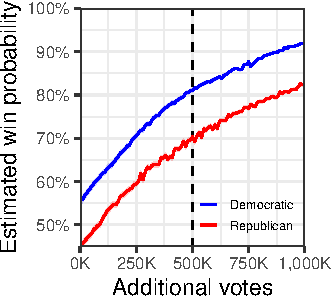
\includegraphics{efficiency.pdf}
  \end{center}
  \caption{\textbf{%
      Estimated probability of winning the election as a function of the number
      of optimized additional votes a candidate receives.%
  }}%
  \label{fig:efficiency}
\end{figure}

\begin{figure}
  \begin{center}
    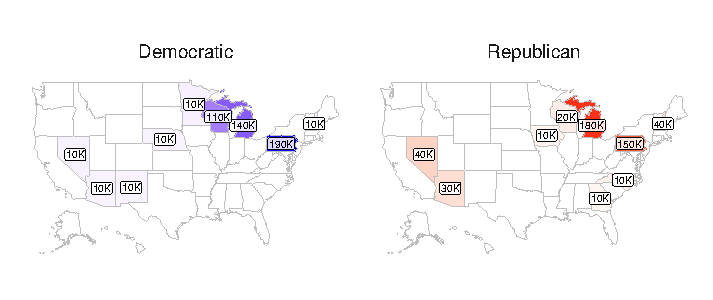
\includegraphics{states.pdf}
  \end{center}
  \caption{\textbf{%
      Strategies requiring 500,000 votes, increasing each party’s probability of
      winning (to 81\% for the Democrats or 70\% for the Republicans), based on
      a forecast conducted a month before the 2024 presidential election.%
  }}%
  \label{fig:states}
\end{figure}

%%%%%%%%%%%%%%%% REFERENCES %%%%%%%%%%%%%%%

\clearpage % Clear all remaining figures and tables then start a new page

% The list of references goes after the main text and before the acknowledgements
% When preparing an initial submission, we recommend you use BibTeX, like this:
%
\bibliography{refs}
\bibliographystyle{sciencemag}

% After the paper has completed peer review and been revised ready for acceptance,
% you should comment out the lines above and copy-paste the contents of your .bbl
% file here instead. This will help ensure that our conversion software works correctly.
% Remember to re-run BibTeX first - check the timestamp!
%
% Example of the first three entries copy-pasted from science_template.bbl:
%
%\begin{thebibliography}{1}
%
%\bibitem{example}
%A.~N. {Author}, An example reference. \emph{Journal of Improbable Research}
%  \textbf{1}, 67 (2020).
%
%\bibitem{example2}
%F.~M. {Surname}, S.~{Author}, A second example. \emph{Interesting Research
%  Letters} \textbf{32}, 897 (2019).
%
%\bibitem{example_preprint}
%P.~{One}, P.~{Two}, P.~{Three}, {An unpublished preprint}. \emph{preprint}
%  (2021), arXiv:2101.12345.
%
%\end{thebibliography}


%%%%%%%%%%%%%%%% ACKNOWLEDGEMENTS %%%%%%%%%%%%%%%

\section*{Acknowledgments}
We thank Stephen Ansolabehere and Marc Meredith for helpful discussions and
feedback. We thank Dan Rosenhack for assistance procuring election simulation
data.
\paragraph*{Funding:}
List the grants, fellowships etc. that funded the research;
use initials to specify which author(s) were supported by each source.
Include grant numbers when appropriate or required by the funding agency.
For example: F.~A. was funded by the Generous Science Agency grant~2372.
\paragraph*{Author contributions:}
All authors contributed equally.
\paragraph*{Competing interests:}
There are no competing interests to declare.
\paragraph*{Data and materials availability:}
All replication materials, data processing code, and analysis code are available
\url{https://github.com/jgaeb/gotv}.


%%%%%%%%%%%%%%%% SUPPLEMENT LIST %%%%%%%%%%%%%%%

% List the contents of your Supplementary Materials, including the numbers of any
% supplementary figures, tables, external data files etc. and any references that are
% cited only in the supplement. In this example, refs. 7-8 are cited only in the supplement.
% Fill out your numbers accordingly and delete any lines that aren't applicable.
\subsection*{Supplementary materials}
Materials and Methods\\
Fig. S1

%%%%%%%%%%%%%%%% END OF MAIN TEXT %%%%%%%%%%%%%%%

\newpage

%%%%%%%%%%%%%%%% START OF SUPPLEMENT %%%%%%%%%%%%%%%

% Figures, tables, equations and pages in the supplement are numbered S1, S2 etc.
\renewcommand{\thefigure}{S\arabic{figure}}
\renewcommand{\thetable}{S\arabic{table}}
\renewcommand{\theequation}{S\arabic{equation}}
\renewcommand{\thepage}{S\arabic{page}}
\setcounter{figure}{0}
\setcounter{table}{0}
\setcounter{equation}{0}
\setcounter{page}{1} % not 0 as \newpage already started a supplementary page
% References continue the numbering from the main text.


%%%%%%%%%%%%%%%% SUPPLEMENT TITLE PAGE %%%%%%%%%%%%%%%

\begin{center}
\section*{Supplementary Materials for\\ \scititle}

% Author list for the supplement
% Indicate the corresponding authors, but do NOT include institutions here
% It would be nice if the template auto-generated this, but doing so is complicated...
Johann D.~Gaebler$^{1,\ast}$,
Andrew Gelman$^{2}$,
Sharad Goel$^{3}$,
Todd Rogers$^{3}$\\
\small$^\ast$Corresponding author. Email: jgaebler@fas.harvard.edu.
\end{center}

% Fill out the numbers for each type of supplementary material,
% and delete any lines that aren't applicable.
% These are just example numbers that don't match the rest of this template.
\subsubsection*{This PDF file includes:}
Materials and Methods\\
Figure S1

\newpage

%%%%%%%%%%%%%%%% MATERIALS AND METHODS %%%%%%%%%%%%%%%

\subsection*{Materials and Methods}

\subsubsection*{Election simulation}

We base our analysis on a simulation of vote totals in the 2024 presidential
election. Our simulation has two components: a model of the joint distribution
of the candidates' voteshares in each state, and a model of the joint
distribution of voter turnout in each state. Combining these two gives simulated
vote totals for each candidate in each state.

\paragraph*{Voteshares.}

To model the candidates' voteshares, we use the \emph{Economist} magazine's 2024
election forecasting model~\cite{gelman2024grappling}. The model predicts the
candidates' likely voteshares in each state based on a combination of national
and state-level polls, prior elections, and economic fundamentals. (For
simplicity, we ignore third parties.) We fit the model using relevant economic
indices and polls as of October 1, 2024, roughly a month before the election.
The model yields a joint distribution of the democratic voteshares in each
state, and, in Maine and Nebraska, each congressional district. We use 10,000
draws from this distribution, which we split into 5,000 training and 5,000
evaluation samples (see below).

\paragraph*{Turnout.}

Since the absolute number of votes a candidate wins by, rather than just the
proportional difference between the candidates' votes, is important for our
analysis, we also model turnout in each state. To do so, we use historical
turnout data from U.S. presidential elections going back to
1976~\cite{mit2017us} and annual estimates of state populations over the same
period~\cite{fred2024}.

We use a simple linear modelling strategy. We first fit a linear regression
predicting the proportion of the US population that turns out to vote in each
presidential election using a linear model with the year as the only predictor.
We then fit a linear regression predicting the proportion of each state's total
population that turns out to vote in each presidential election using a linear
model with year and national turnout proportion as predictors.

To simulate the joint distribution of turnout in each state, we first draw a
sample of 10,000 years from the fitted normal distribution of the national turnout
proportion in 2024, which we propagate using the state-level models to obtain
samples of turnout proportion in each state, which we then multiply by the
state's population in 2024. We again split the sample into 5,000 training and
5,000 evaluation samples.

\paragraph*{Harmonization.}

To produce samples of vote totals, we simply scale the voteshares in each state
by the corresponding turnout sample. Because the boundaries of congressional
districts shift between 1976 and 2024, however, directly modeling turnout at the
level of congressional districts is more difficult, so we only model turnout at
the state level. To produce estimated vote totals for congressional districts in
Maine and Nebraska, we calculate the congressional district turnouts that are
both consistent with the state-level turnout and voteshare samples and the
congressional district-level voteshare samples. In Maine, which has two
congressional districts, this uniquely determines total turnout in each
district; in Nebraska, which has three congressional districts, it does not.
Consequently, we additionally choose the unique solution minizing the sum of
squared differences between sampled and actual district-level turnout in the
2024 election.

\subsubsection*{Optimizing campaign strategies}

To find efficient strategies for each party, we represent the problem as a
mixed-integer program (``MIP''), which we solve numerically.

\paragraph*{Problem formulation.}

Let \(k = 56\) denote the number of distinct states and congressional districts
in the US (that is, all 50 states, Washington~D.C., the two congressional
districts in Maine, and the three congressional districts in Nebraska), let
\(\bb e \in \B R^k\) denote the vector of corresponding electoral votes, and let
\(\bb t \in \B N^k\) denote the vector of corresponding actual turnouts in the
2024 election. Let \(N\) denote the number of samples from our simulation of
vote totals. (We use \(N = 500\) in our MIPs.) Let \(\bb T \in \B R^{N \times
k}\) denote the matrix of simulated turnout samples, and let \(\bb V \in [0,
1]^{N \times k}\) denote the matrix of simulated Democratic voteshares. (To find
optimal strategies for the Republican party, we simply replace \(V_{i,j}\) with
\(1 - V_{i,j}\) for all \(i\) and \(j\).) Let \(\bb x \in \B R^k\) denote the
additional votes the party of interest receives in each state or congressional
district \emph{if} they deploy resources there. Let \(\bb y \in \{0, 1\}^k\)
denote \emph{whether} a party deploys resources in the corresponding state or
congressional district. Let \(\bb W \in \{0, 1\}^{N \times k}\) denote whether
the strategy results in a win for the party of interest in a given sample and
district, and let \(\bb z \in \{0, 1\}^N\) denote whether the strategy results
in a win for the party of interest in the corresponding sample. Then, our goal
is to find a strategy \(\bb x \cdot \bb y\) requiring at most \(B\) additional
votes that maximizes the number of samples in which the party of interest wins
the election. (For notational simplicity, we assume throughout that scalar
operations on vectors and matrices are performed elementwise.)

These relations can all be expressed linearly in the form of a MIP as follows.
First, our objective can be expressed as follows:
\begin{equation}
\label{eq:objective}
  \begin{array}{ll}
    \text{maximize} & \bb 1^\top \bb z \\
    \text{where} & \bb x \in \B R^k, \bb y \in \{0, 1\}^k, \bb W \in
    \{0, 1\}^{N \times k}, \bb z \in \{0, 1\}^N.
  \end{array}
\end{equation}
To ensure that \(\bb x\) represents a proportion of votes, we impose a
non-negativity constraint:
\begin{equation}
\label{eq:nonnegativity}
  \bb x \geq \bb 0.
\end{equation}
To ensure that \(\bb W\) captures whether a state or congressional district is
won, we require that the votes deployed by the strategy there (i.e., \(x_j \cdot
y_j\)) plus the votes already received by the Democratic party in that state or
district (i.e., \(V_{i,j} \cdot T_{i,j}\)) exceeds one half of the total votes
cast in that state or district (i.e., \(T_{i,j} / 2\)) if the party of interest
wins the election in that state or district:
\begin{equation}
\label{eq:win}
  \bb V + \bb 1 (\bb x \cdot \bb y)^\top \operatorname{/} \bb T \geq \frac 1 2
  \cdot \bb W.
\end{equation}
To ensure that \(\bb z\) captures whether the strategy results in an overall win
for the Democratic party, we require that the sum of electoral votes in states
or congressional districts won exceeds 269, one half of the total electoral
votes, if the party of interest wins the election in that sample:
\begin{equation}
\label{eq:electoral}
  \bb W \bb e \geq 270 \cdot \bb z.
\end{equation}
We cap the number of votes deployed in each state or congressional district at
5\% of the actual turnout in that state or district:
\begin{equation}
\label{eq:cap}
  \bb x \leq \frac 1 {20} \cdot \bb t.
\end{equation}
Additionally, we require that at least 10,000 votes are deployed in any state or
congressional district where resources are deployed:
\begin{equation}
\label{eq:minimum}
  x_j \geq 10,000 \quad \text{for \(j\) such that \(t_j \geq 200,000\)}; \qquad
  y_j = 0 \quad \text{otherwise}.
\end{equation}
(The second alternative in Eq.~\eqref{eq:minimum} is required for districts with
low turnout, as otherwise the constraints in Eq.~\eqref{eq:cap} and
Eq.~\eqref{eq:minimum} would be contradictory.) To capture the nested structure
of the congressional districts in Maine and Nebraska, we require that the votes
deployed in the state as a whole are equal to the sum of the votes deployed
in the congressional districts:
\begin{equation}
\label{eq:congressional}
  x_{j_{\text{ME}}} = x_{j_{\text{ME-1}}} + x_{j_{\text{ME-2}}} \qquad
  \text{and} \quad x_{j_{\text{NE}}} = x_{j_{\text{NE-1}}} + x_{j_{\text{NE-2}}}
  + x_{j_{\text{NE-3}}},
\end{equation}
where \(j_{\text{ME}}\) and \(j_{\text{NE}}\) denote the indices of Maine and
Nebraska, respectively, and \(j_{\text{ME-1}}\), \(j_{\text{ME-2}}\),
\(j_{\text{NE-1}}\), \(j_{\text{NE-2}}\), and \(j_{\text{NE-3}}\) denote the
indices of their congressional districts. Finally, we constrain the total number
of votes deployed to at most \(B\):
\begin{align}
\label{eq:budget}
  \begin{split}
  B &\leq \bb 1^\top \bb x - y_{j_{\text{ME}}} \cdot \left(y_{j_{\text{ME-1}}}
     \cdot x_{j_{\text{ME-1}}} + y_{j_{\text{ME-2}}} \cdot
     x_{j_{\text{ME-2}}}\right) \\
    &\qquad\qquad - y_{j_{\text{NE}}} \cdot \left(y_{j_{\text{NE-1}}} \cdot
      x_{j_{\text{NE-1}}} + y_{j_{\text{NE-2}}} \cdot x_{j_{\text{NE-2}}} +
      y_{j_{\text{NE-3}}} \cdot x_{j_{\text{NE-3}}}\right).
  \end{split}
\end{align}
(We subtract the votes deployed in congressional districts in Maine and Nebraska
from the total number of votes when calculating the budget, as these votes are
already included in the state totals if the state as a whole is won.)

We note that the the products of \(\bb x\) and \(\bb y\) in Eq.~\eqref{eq:win}
and of components of \(\bb y\) in Eq.~\eqref{eq:cap} appear nonlinear. However,
since \(\bb y\) is binary, they can be expressed as linear constraints by the
introduction of auxiliary variables and constraints. For instance, in the former
case, we can introduce \(\bb p\) satisfying
\[
  \bb p \geq 0, \qquad \bb p \leq \bb x, \qquad \bb p \leq M \cdot \bb y,
\]
where \(M\) is a sufficiently large constant. Likewise, we can replace products
of the form \(y_i \cdot y_{i'}\) with an auxiliary binary variable \(q\) satisfying
\[
  q \geq 0, \quad q \leq y_i, \quad q \leq y_{i'}, \quad q \geq y_i + y_{i'} -
  1.
\]
See, e.g.,~\cite{brown2007formulating} for additional details.

\paragraph*{Implementation.}

We implement the MIP described in Eqs.~\eqref{eq:objective}--\eqref{eq:budget}
in julia using the \texttt{JuMP} package~\cite{dunning2017jump}, which we solve
using the \texttt{Gurobi} solver~\cite{gurobi2024}, solving each problem
instance to optimality. We draw 10 random samples of size 500 from the 5000
training samples of voteshares and turnout, and solve the MIP for each party and
sample across a grid of budgets ranging from 10,000 to 1,000,000 additional
votes in increments of 10,000. We then evaluate the out-of-sample performance of
the strategies on the remaining 4,500 samples of voteshares and turnout in the
evaluation set. For each number of additional votes, we select the strategies
that maximize the number of samples in which the Democratic (resp., Republican)
party wins the election out of sample. Finally, we re-evaluate the strategies on
the full set of 5,000 evaluation samples, computing normal 95\% confidence
intervals for the resulting win probabilities. These are the values reported in
Fig.~\ref{fig:efficiency} and Fig.~\ref{fig:states}.

\newpage

%%%%%%%%%%%%%%%% SUPPLEMENTARY FIGURES %%%%%%%%%%%%%%%

\begin{figure} % Do not use \begin{figure*}
  \begin{center}
    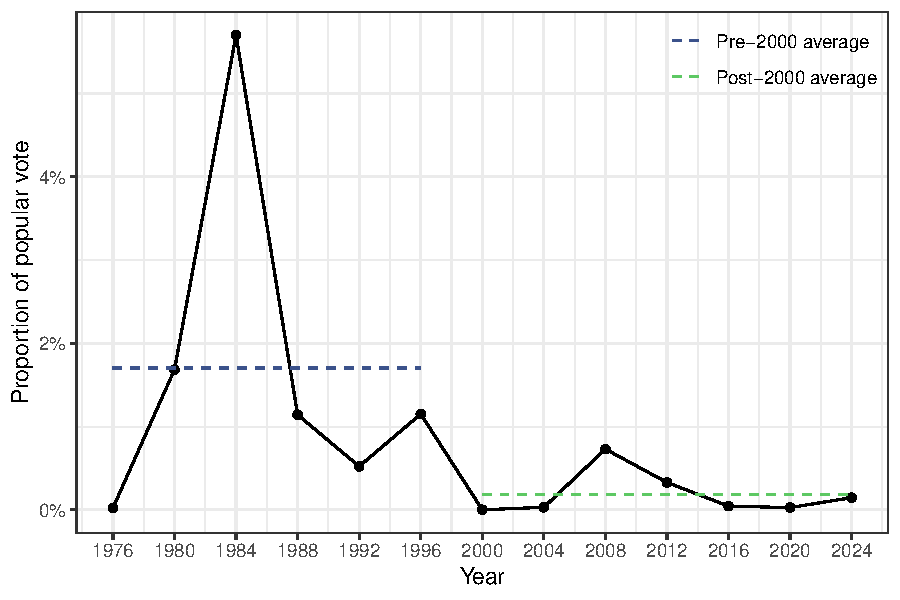
\includegraphics{margin.pdf}
  \end{center}
	\caption{%
    \textbf{Minimum numbers of votes required to swing presidential elections
    since 1976.} Dashed blue and green lines indicate the average minimum number
    of votes required to swing the election before and after 2000, respectively.
    With the exception of the 1976 election, which could have been swung by
    roughly 7,000 votes in Hawaii and 11,000 votes in Ohio, substantially fewer
    votes would have been required to swing the 2000 and subsequent presidential
    elections than elections in decades prior.%
  }%
\label{fig:margin}
\end{figure}

\end{document}
% End of science_template.tex
